\documentclass[12pt,A4]{article}

\usepackage[utf8]{inputenc}
\usepackage{comment}
\usepackage[english]{babel}
\usepackage{graphicx}
\usepackage{blindtext}
\usepackage{subfiles} 
\usepackage{blindtext}
\usepackage[T1]{fontenc}
\usepackage{xcolor}
\usepackage{hyperref}
\usepackage{biblatex}

\graphicspath{{./figures/}}

\addbibresource{ref.bib}

\title{cloud robot}
\author{robot team}
\date{9 2020}

\addcontentsline{toc}{section}{Abstract}
\addcontentsline{toc}{section}{list of figures}
\addcontentsline{toc}{section}{list of tables}

\begin{document}

\begin{titlepage}
\maketitle
\end{titlepage}

%example for an image

\includegraphics[width=0.9\textwidth]{image1}
%

\tableofcontents

\subfile{chapters/abstract}

%list of figures 
\listoffigures
%list of tables
\listoftables
%list of abbreviation 


\subfile{chapters/chapter1}
\subfile{chapters/chapter2}
\subfile{chapters/chapter3}
\subfile{chapters/chapter4}
\subfile{chapters/chapter5}
\subfile{chapters/chapter6}

%example for a figure 
\begin{figure}
    \centering
    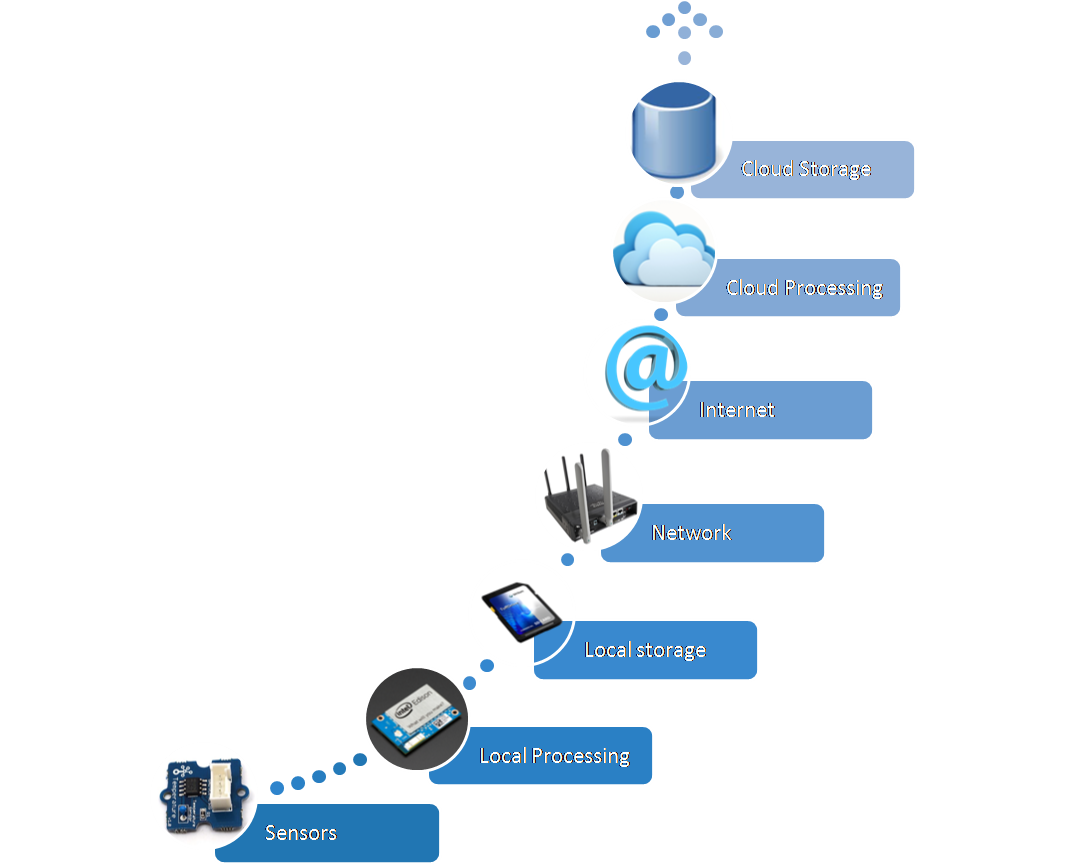
\includegraphics[width=0.3\textwidth]{IOT}
    \caption{IOT}
\end{figure}
%

\printbibliography


\end{document}

